\section{Theorie}
\label{sec:Theorie}

\subsection{Aufbau des Geiger-Müller Zählrohres}
Im wesentlichen besteht das Geiger-Müller Zählrohr aus 4 Komponenten.\\
Das Rohr selbst ist ein metallisch leitender \textit{Zylinder} mit abgedichtetem Boden.
Das andere Ende ist eine Membran aus \textit{Mylar}.\\
Der Hohlraum ist komplett mit einem \textit{Gasgemisch}, meistens Argon und Ethylalkohol, gefüllt.
In der Mitte des Rohres ist ein \textit{Metallstab}, der als Anodendraht wirkt.
Die Kathode ist der Zylinder.\\
An den entstehenden zylindrischen Kondensator wird eine Spannung von $300\si{\volt}\ -\ 2000\si{\volt}$ angelegt.\\
\autoref{fig:kern} zeigt einen Querschnitt des Geiger-Müller Zählrohres.

\begin{figure}[htbp]
    \centering
    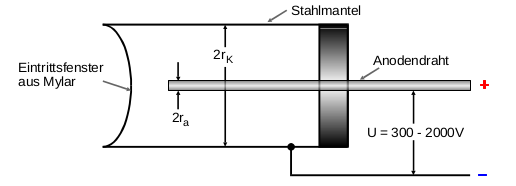
\includegraphics[scale=0.7]{Pics/quer.png}
    \caption{Querschnitt eines Geiger-Müller Zählrohres.}
    \label{fig:kern}
\end{figure}

\subsection{Funktionsweise eines Zählrohres}
Das Geiger-Müller Zählrohr ist dazu da, um radioaktive Strahlung zu messen und die Intensität zu ermitteln.\\
Tritt ein $\alpha$- oder $\beta$-Teilchen oder ein Röntgen- oder Gammaquant in den Hohlraum des Rohrs ein, so ionisiert es die Gasatome darin.
Das dadurch frei werdende Elektron wird im elektrischen Feld des Kondensators zum Anodendraht hingezogen, wo es beim Auftreffen einen elektrischen Impuls erzeugt.
Über elektrische Schaltkreise, die ans Zählrohr angeschlossen sind, lässt sich dieser Impuls messen.
\subsubsection{Verhalten der Elektron-Ion Paare bei steigender Spannung}
\autoref{fig:verlauf1} zeigt den Verlauf der Ionisation mit zunehmender Spannung am Zählrohr.

\begin{figure}[htbp]
    \centering
    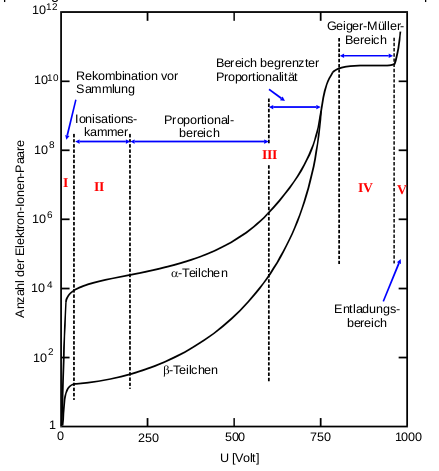
\includegraphics[scale=0.7]{Pics/verlauf.png}
    \caption{Verlauf der Anzahl von Elektron-Ion Paaren mit zunehmender Spannung, mit den jeweiligen Bereichen.}
    \label{fig:verlauf1}
\end{figure}

Die Energie des einfallenden Teilchens ist proportional zu der Anzahl an ionisierten Teilchen im Gas.
Allerdings hängen die weiteren Verläufe der gelösten Elektronen stark von der Zählrohrspannung ab.
Der erste Bereich von 0 - 50 Volt zeigt, dass die entkoppelten Elektronen zu schwach sind, sodass sie rekombinieren bevor sie den Anodendraht erreichen.\\
Steigt die Spannung weiter an, verhält sich der Ionisationsstrom proportional zur Energie der einfallenden Teilchen.
Da solche Ströme sehr gering sind, ist es nur bei sehr hoher Strahlungsbelastung effektiv das Zählrohr mit solcher Spannung zu nutzen.
Der assoziierte Bereich ist der II auf \autoref{fig:verlauf1}.\\
Wird nun die Spannung weiter erhöht, könne die ionisierten Elektronen ihrerseits Gasatome ionisieren, dessen Elektron das ebenfalls können.
Dadurch steigt die Anzahl an ionisierten Paaren exponentiell an und die Ladungsmenge $Q$ ist nun so groß, dass sie einen messbaren elektrischen Impuls in der Drahtanode erzeugen kann.
Hierbei sind noch alle erzeugten Elektronen proportional an die Energie des radioaktiven Teilchens gebunden.
Daher wird dieser Bereich (Bereich III in \ref{fig:verlauf1}) Proportionalbereich genannt.\\
Ab einer Spannung von ca $750\si{\volt}$ entfällt die Proportionalität und es ist nur noch eine Intensitätsmessung möglich.
Ab dieser Energie können ionisierte Elektronen UV-Strahlung durch Einfallen in Argon-Atome erzeugen.
Diese kann ihrerseit ebenfalls ionisieren, sodass sich über das gesamte Volumen des Rohres Elektronen verteilen und den Anodendraht überall erreichen.
Die Ladung am Draht hängt nur vom Volumen des Zählrohres und der angelegten Spannung ab.
Hierbei muss die Elektrik keinen großen Aufwand erbringen, um den Impuls an der Anode nachzuweisen.
Dieser Bereich wird Geiger-Müller Bereich genannt, da hier der primäre Nutzen des Gerätes liegt.
\subsubsection{Totzeit}
Während beim Entladen (Bereich V in \ref{fig:verlauf1}) die Elektronen durch ihre geringe Masse sehr schnell die Anode erreichen, brauchen die positiv geladenen Atomkerne länger.
Daraus resultiert ein sog. Ionenschlauch, der das elektrische Feld
\begin{equation}
    E\left(r\right) = \frac{U}{r\cdot \ln\left(\frac{r_k}{r_a}\right)}
\end{equation}
um den Draht stark abschwächt.
Während dieser Zeit ist keine Stoßionisation möglich und infolge dessen wird kein Teilchen registriert.\\
Dieser Zeitabschnitt wird \textit{Totzeit} genannt.\\
Auf die Totzeit folgt die Erholungszeit des Zählrohres, da es dauert bis das ursprüngliche elektrische Feld wieder maximal stark ist.
In dieser Erholungszeit entstehen Sekundärelektronen, beim Auftreffen der Kerne auf der Kathode.
Diese Elektronen können das gesamte elektrische Feld durchqueren und mehrmals die Zählrohrentladung erneut zünden.
Dies wird Nachentladungen genannt.\\
Die Bestimmung der Totzeit erfolgt mit der zwei Quellen Methode.
Die resultierende Gleichung ist:
\begin{equation}
    T \approx \frac{N_1\ +\ N_2\ -\ N_{1+2}}{2N_1N_2}
    \label{eq:tot}
\end{equation}

\subsection{Charakteristik des Zählrohres}
Eine Charakteristik ist die Anzahl der Impulse gegen die Zählrohrspannung aufgetragen.
Dabei beginnt der Auslösebereich bei $U_E$.
Nach dem Auslösebereich folgt ein Plateau.
Idealerweise müsste es die Steigung null haben, jedoch erzeugen Nachentladungen eine leichte Steigung.
Nach dem Plateau beginnt die Dauerentladung.
Dies ist in \autoref{fig:platt} dargestellt.

\begin{figure}[htbp]
    \centering
    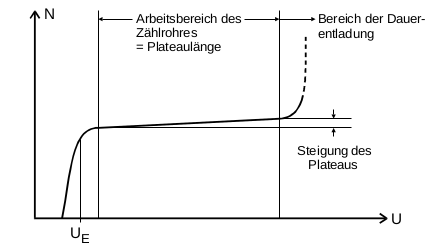
\includegraphics[scale=0.7]{Pics/charakter.png}
    \caption{Verlauf der Impulse bei zunehmender Spannung.}
    \label{fig:platt}
\end{figure}

\subsection{Zählrohrstrom}
Für die Ermittlung der freigesetzten Ladungen $Z$ pro einfallendem Teilchen benötigt es die Impulsanzahl, sowie den gemessenen Strom über das Zählrohr.
Die Ladungen werden dann gemäß \ref{eq:charge} berechnet.
\begin{equation}
    Z = \frac{I}{e_0N}
    \label{eq:charge}
\end{equation}